% 04-trien-khai.tex — Chương 4: Cách thức triển khai và vận hành

\chapter{Cách thức triển khai và vận hành}\label{ch:trienkhai}


\section{Kiến trúc tổng thể}

Hệ thống được xây dựng theo kiến trúc nhiều tầng, chạy hoàn toàn trong các container trên máy chủ nội bộ,
dùng chung cơ sở dữ liệu PostgreSQL~\cite{postgresdocs} của đơn vị. Bộ điều phối công việc Apache Airflow~\cite{airflowdocs} là ``người điều hành lịch'': kích hoạt từng khâu đúng giờ, ghi nhật ký, thử lại khi lỗi.

\begin{figure}[!ht]
\centering
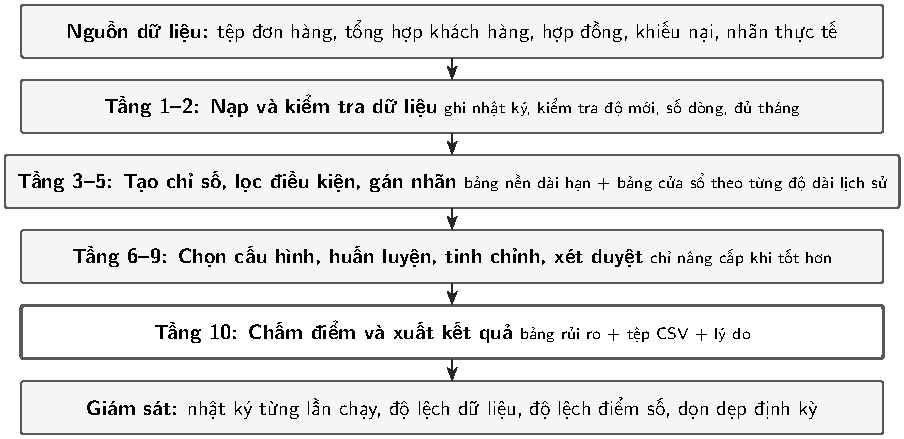
\includegraphics[width=434.0bp]{figures/fig05.pdf}
\caption{Kiến trúc nhiều tầng của hệ thống}\label{fig:kientruc}
\end{figure}

Dữ liệu được tổ chức thành các ``ngăn'' riêng trong cơ sở dữ liệu, mỗi ngăn một mục đích:

{\tablefont
\begin{longtable}{@{}L{3.6cm}>{\raggedright\arraybackslash}p{12.03cm}@{}}
\caption{Cách tổ chức dữ liệu trong cơ sở dữ liệu}\label{tab:schema}\\
\toprule
\hdrrow\hh{Ngăn dữ liệu} & \hh{Chứa gì}\\
\midrule
\endfirsthead
\toprule
\hdrrow\hh{Ngăn dữ liệu} & \hh{Chứa gì}\\
\midrule
\endhead
\bottomrule
\endfoot
Dữ liệu nguồn & Đơn hàng theo tháng, tổng hợp khách hàng, thông tin hợp đồng, khiếu nại, danh sách tệp đã nạp.\\
\rowa Nhật ký nạp dữ liệu & Trạng thái từng lần nạp, kết quả kiểm tra độ mới và đầy đủ.\\
Dữ liệu nền dài hạn & Tổng hợp lịch sử từng khách đến từng mốc; cấu hình mô hình tốt nhất; bảng rủi ro kết quả.\\
\rowa Dữ liệu cửa sổ & Các bảng chỉ số hành vi theo từng độ dài lịch sử được thử (3, 4, 5\ldots tháng).\\
Giám sát & Nhật ký chạy, độ lệch đặc trưng, độ lệch điểm số.\\
\end{longtable}}
\vspace{4pt}

\section{Lịch vận hành tự động}

Toàn bộ công việc được khai báo thành các luồng công việc DAG trong Airflow. Luồng này kích hoạt luồng kia nên không cần người ngồi bấm nút.

{\tablefont
\begin{longtable}{@{}L{4.4cm}L{3.0cm}>{\raggedright\arraybackslash}p{7.81cm}@{}}
\caption{Các luồng công việc tự động}\label{tab:dag}\\
\toprule
\hdrrow\hh{Luồng công việc} & \hh{Lịch chạy} & \hh{Nhiệm vụ}\\
\midrule
\endfirsthead
\toprule
\hdrrow\hh{Luồng công việc} & \hh{Lịch chạy} & \hh{Nhiệm vụ}\\
\midrule
\endhead
\bottomrule
\endfoot
Nạp dữ liệu  & Hằng ngày, & Quét tệp mới, chuẩn hóa, nạp vào cơ sở dữ liệu, kiểm tra rồi kích hoạt bước tạo chỉ số.\\
\rowa Tạo chỉ số & Tự kích hoạt sau khi nạp xong; có thể chạy tay khi cần bù dữ liệu & Sinh bảng nền dài hạn và bảng chỉ số cửa sổ; kích hoạt bước tiếp theo.\\
Chuẩn bị mô hình  & Tự kích hoạt sau khi tạo chỉ số & Bảo đảm có mô hình sẵn sàng rồi kích hoạt chấm điểm.\\
\rowa Chấm điểm và gửi danh sách  & Hằng ngày, tự kích hoạt sau bước chuẩn bị; có thể chạy tay & Dự đoán khách hàng có nguy cơ rời bỏ bằng mô hình hiện tại, xuất danh sách mới nhất và gửi cho bộ phận chăm sóc khách hàng; không huấn luyện lại.\\
Huấn luyện lại  & Theo chu kỳ, thiết kế khi đủ dữ liệu nhất định & Huấn luyện ứng viên mới, tinh chỉnh, chỉ thay thế mô hình hiện tại nếu tốt hơn.\\
\rowa Dọn dẹp  & 03:00 ngày mùng 1, mỗi quý một lần & Dọn mô hình, nhật ký, tệp cũ theo thời hạn lưu trữ.\\
\end{longtable}}
\vspace{4pt}

Việc dự đoán và gửi danh sách được chạy hằng ngày, còn việc huấn luyện lại không gắn với lịch cố định:
chu kỳ sẽ được thiết kế khi đã tích lũy đủ dữ liệu, dự kiến 3 ngày hoặc 1 tuần một lần. Trong thời gian đó, hệ thống tiếp tục dùng mô hình hiện tại để chấm điểm hằng ngày.

\begin{figure}[!ht]
\centering
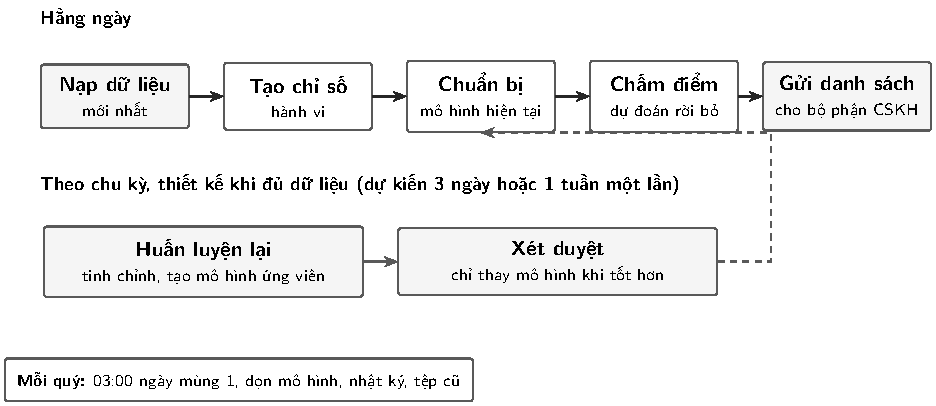
\includegraphics[width=\textwidth]{figures/fig06.pdf}
\caption{Nhịp vận hành: dự đoán và gửi danh sách hằng ngày, huấn luyện lại theo chu kỳ}\label{fig:nhip}
\end{figure}

\section{Cơ chế bảo vệ chất lượng cổng xét duyệt mô hình}

Đây là một thiết kế quan trọng với người quản lý: hệ thống không tự động thay mô hình chỉ vì có mô hình mới.

\begin{figure}[!ht]
\centering
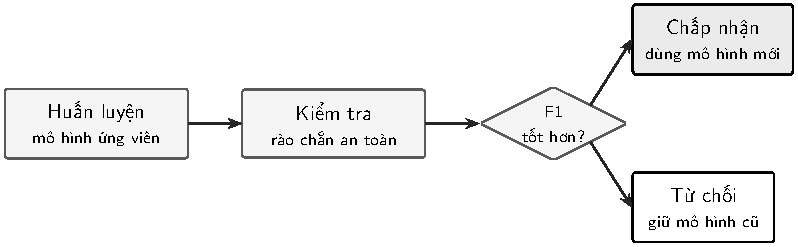
\includegraphics[width=383.1bp]{figures/fig07.pdf}
\caption{Quy trình xét duyệt mô hình trước khi đưa vào sử dụng}\label{fig:duyet}
\end{figure}

Quy tắc cụ thể:

\begin{itemize}
  \item Lần chạy đầu tiên: chấp nhận mô hình để có sản phẩm sử dụng.
  \item Các lần sau: chấp nhận khi điểm F1 cải thiện so với mô hình đang dùng, hoặc khi đến chu kỳ buộc làm mới.
  \item Từ chối và giữ mô hình cũ: khi các rào chắn dữ liệu thất bại hoặc tỷ lệ khách rời bỏ trong nhãn quy tắc bất thường.
\end{itemize}

Nhờ vậy, ngay cả khi dữ liệu tháng nào đó bị lỗi, danh sách kết quả vẫn được tạo từ mô hình đã được kiểm chứng trước đó, không bị gián đoạn và không bị sai lệch.

\section{Giám sát và kiểm toán}

{\tablefont
\begin{longtable}{@{}L{3.4cm}>{\raggedright\arraybackslash}p{12.23cm}@{}}
\caption{Các lớp giám sát}\label{tab:giamsat}\\
\toprule
\hdrrow\hh{Lớp giám sát} & \hh{Giám sát điều gì và để làm gì}\\
\midrule
\endfirsthead
\toprule
\hdrrow\hh{Lớp giám sát} & \hh{Giám sát điều gì và để làm gì}\\
\midrule
\endhead
\bottomrule
\endfoot
Nhật ký từng lần chạy & Ghi mã lần chạy, thời gian, trạng thái, độ dài lịch sử cũ/mới, điểm F1 ứng viên, kết quả chấp nhận hay từ chối, có huấn luyện/chấm điểm hay không. Dùng để truy vết khi cần giải trình.\\
\rowa Độ lệch điểm số & Theo dõi từng tháng: số khách hoạt động, số khách rủi ro, tỷ lệ rủi ro, mức điểm trung bình và các mốc phân vị. Phát hiện danh sách đột nhiên ``phình'' hoặc ``xẹp''.\\
Độ lệch dữ liệu & So sánh phân phối từng chỉ số tháng mới với hồ sơ lúc huấn luyện. Cảnh báo khi hành vi khách hàng hoặc chất lượng dữ liệu thay đổi mạnh.\\
\rowa Cấu hình mô hình & Lưu độ dài lịch sử tốt nhất, ngưỡng cảnh báo, thước đo, nguồn kiểm tra, lịch sử chấp nhận/từ chối.\\
Gói mô hình & Lưu cùng nhau: mô hình, danh sách chỉ số, hồ sơ chỉ số, cấu hình lọc điều kiện. Đảm bảo chấm điểm dùng đúng cấu hình đã học.\\
\rowa Dọn dẹp định kỳ & Giữ hệ thống gọn; tránh đầy ổ đĩa do tệp tạm và nhật ký cũ.\\
\end{longtable}}
\vspace{4pt}

\begin{hieunhanh}[PSI và KS là gì?]
Là hai phép đo độ lệch của dữ liệu~\cite{siddiqi2006scorecards,massey1951ks,gama2014drift}. Nếu số liệu tháng này khác hẳn số liệu mà mô hình từng học ví dụ do đổi cách ghi nhận dữ liệu, hoặc do thị trường biến động mạnh, hệ thống sẽ ghi nhận để con người kiểm tra trước khi tin vào kết quả.
\end{hieunhanh}

\section{Hạ tầng và cài đặt}

\subsection{Thành phần hạ tầng}

{\tablefont
\begin{longtable}{@{}L{4.2cm}>{\raggedright\arraybackslash}p{11.43cm}@{}}
\caption{Các thành phần hạ tầng của hệ thống}\label{tab:haitang}\\
\toprule
\hdrrow\hh{Thành phần} & \hh{Vai trò}\\
\midrule
\endfirsthead
\toprule
\hdrrow\hh{Thành phần} & \hh{Vai trò}\\
\midrule
\endhead
\bottomrule
\endfoot
Cơ sở dữ liệu PostgreSQL nghiệp vụ & Chứa dữ liệu nguồn, chỉ số, mô hình và kết quả.\\
\rowa Cơ sở dữ liệu quản lý của Airflow & Một cơ sở dữ liệu riêng chỉ để Airflow lưu trạng thái công việc, tách biệt với dữ liệu nghiệp vụ.\\
Máy chủ giao diện/API Airflow & Màn hình quản trị luồng công việc cho người vận hành.\\
\rowa Bộ lập lịch & Quyết định công việc nào chạy khi nào.\\
Bộ đọc luồng công việc & Đọc và kiểm tra các tệp mô tả luồng.\\
\rowa Bộ kích hoạt & Xử lý việc ``luồng này chờ luồng kia'' hoặc kích hoạt luồng nối tiếp.\\
Kho ảnh đóng gói nội bộ & Lưu phiên bản đóng gói của hệ thống để triển khai lặp lại và hoàn tác được.\\
\end{longtable}}
\vspace{4pt}

Hệ thống được đóng gói trên nền Airflow phiên bản 3.1.7; giao diện quản trị được đặt tại địa chỉ \texttt{ai.vnpost.vn/airflow-churn}.
Việc đóng gói theo container~\cite{dockerdocs} giúp sao chép môi trường sang máy chủ khác, nâng cấp hoặc quay lại phiên bản trước một cách nhanh chóng và có kiểm soát.

\subsection{Khi thay đổi cần làm gì}

{\tablefont
\begin{longtable}{@{}L{5.4cm}>{\raggedright\arraybackslash}p{10.23cm}@{}}
\caption{Hướng dẫn nhanh khi có thay đổi}\label{tab:thaydoi}\\
\toprule
\hdrrow\hh{Thay đổi} & \hh{Cần làm}\\
\midrule
\endfirsthead
\toprule
\hdrrow\hh{Thay đổi} & \hh{Cần làm}\\
\midrule
\endhead
\bottomrule
\endfoot
Thêm thư viện hoặc đổi cấu hình đóng gói & Đóng gói lại phiên bản mới và khởi động lại các thành phần.\\
\rowa Sửa mã chương trình hoặc luồng công việc & Thường không cần đóng gói lại vì mã được gắn trực tiếp; chờ bộ lập lịch nạp lại.\\
Đổi biến môi trường & Tạo lại các thành phần để cấu hình mới có hiệu lực.\\
\rowa Đổi cách tính chỉ số & Chạy lại luồng tạo chỉ số.\\
Đổi quy tắc nhãn, mô hình, tinh chỉnh & Chạy lại luồng huấn luyện để tạo mô hình mới.\\
\end{longtable}}
\vspace{4pt}

\section{An toàn và bảo mật dữ liệu}

\begin{itemize}
  \item Mã hóa định danh: mã khách hàng và mã bưu gửi được mã hóa ánh xạ một-một ngay từ khâu cung cấp dữ liệu; hệ thống làm việc với mã đã mã hóa.
  \item Giới hạn chạy nội bộ: hệ thống chạy trên hạ tầng của Tổng công ty, dùng cơ sở dữ liệu nội bộ; thông tin kết nối được quản lý bằng tệp cấu hình môi trường, không nằm trong mã chương trình.
  \item Tách biệt cơ sở dữ liệu: dữ liệu quản trị của Airflow tách khỏi dữ liệu nghiệp vụ.
  \item Truy vết: mọi lần chạy đều có nhật ký; mô hình và cấu hình được lưu theo phiên bản.
\end{itemize}